\section{System Design}\label{sec:design}

\begin{figure*}[t]
  \centering
  % If the figure is too tall, switch to height=0.33\textheight (or similar).
  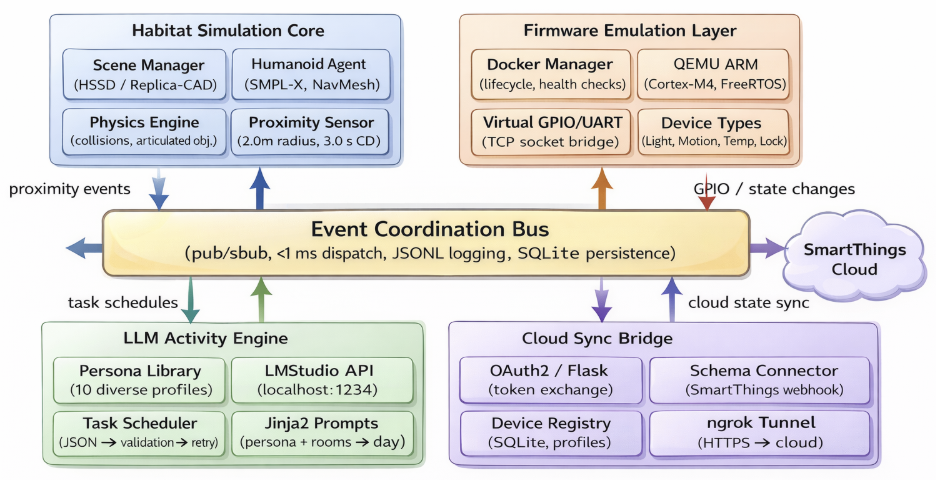
\includegraphics[width=\textwidth]{figures/architecture.png}
  \caption{Architecture of \sys{}. Seven functional layers communicate through a central publish-subscribe event coordination bus. Double-headed arrows denote bi-directional real-time data flow. The Cloud Sync Bridge connects to Samsung SmartThings via an ngrok HTTPS tunnel.}
  \label{fig:architecture}
\end{figure*}



\sys{} comprises seven layers (\Cref{fig:architecture}):
the \emph{Habitat Simulation Core}, the \emph{Firmware Emulation
Layer}, the \emph{LLM Activity Engine}, the \emph{Cloud Sync
Bridge}, the \emph{Event Coordination Bus}, the \emph{Simulated
Home Network}, and the \emph{Security Testing Layer}.

\subsection{Habitat Simulation Core}

The simulation core wraps Meta Habitat~3.0 to provide:
\begin{itemize}[leftmargin=*]
  \item \textbf{Scene management.}  HSSD~\cite{hssd} and Replica-CAD scene
    datasets supply photorealistic room layouts with furniture and
    appliance meshes.
  \item \textbf{Humanoid agents.}  SMPL-X parametric humanoid models
    navigate rooms, interact with objects (e.g., opening doors,
    picking up items), and trigger device proximity events.
  \item \textbf{Physics engine.}  Bullet physics provides collision
    detection and object manipulation, enabling realistic interactions
    between humanoids and IoT-instrumented objects.
\end{itemize}

\subsection{Firmware Emulation Layer}\label{sec:firmware-layer}

Each simulated IoT device is backed by a Docker container running
QEMU~10.2 in ARM system-emulation mode targeting the
\textbf{LM3S6965EVB} evaluation board (ARM Cortex-M3, Thumb ISA).
Unlike prior IoT testbeds that use host-side mocks, \sys{} executes
\emph{real} bare-metal firmware---compiled from C with
\texttt{arm-none-eabi-gcc}---inside QEMU's instruction-accurate
emulator, preserving interrupt semantics, register state, and
memory layout (though not cycle-level timing).

\paragraph{Per-Device Firmware Variants.}
We provide six firmware images, each implementing a device-specific
command set and sensor model:
\begin{enumerate}[leftmargin=*]
  \item \textbf{Smart Light} --- PWM brightness (0--100\%), color
    temperature (2\,700--6\,500\,K), on/off/toggle.
  \item \textbf{Motion Sensor} --- PIR interrupt with configurable
    sensitivity (1--10) and cooldown timer.
  \item \textbf{Temperature Sensor} --- ADC sampling at 1\,Hz with
    Kalman filtering and threshold alerts.
  \item \textbf{Humidity Sensor} --- relative-humidity and
    temperature combo sensor with calibration.
  \item \textbf{Door Sensor} --- magnetic contact with
    open/closed state and tamper detection.
  \item \textbf{Smart Plug} --- relay-driven outlet with power
    metering (watts) and scheduling.
\end{enumerate}
All six variants share a common skeleton (ISR vector table, UART
driver, command dispatcher) and are compiled with identical flags
(\texttt{-mcpu=cortex-m3 -mthumb -Os -nostartfiles -nostdlib}).
A custom linker script places the ISR vector in \texttt{.isr\_vector}
and allocates 64\,KB flash / 20\,KB SRAM, matching the physical
LM3S6965 memory map.

\paragraph{UART Protocol.}
Firmware communicates with the host through UART0 mapped to a TCP
socket (\texttt{-serial tcp::15000,server,nowait}).  The protocol
uses newline-terminated ASCII commands:
\begin{itemize}[leftmargin=*]
  \item \texttt{IDENTIFY} / \texttt{ID} --- returns device type,
    capabilities, firmware version, and unique ID.
  \item \texttt{ON}, \texttt{OFF}, \texttt{TOGGLE},
    \texttt{STATUS}, \texttt{GET\_ALL} --- power and state control.
  \item \texttt{SET\_ID}, \texttt{AUTH} --- device provisioning and
    token-based authentication.
  \item \texttt{FW\_UPDATE:<hex>}, \texttt{FW\_APPLY} --- over-the-air
    firmware update (intentionally unauthenticated).
  \item \texttt{DEBUG\_DUMP} --- diagnostic command that leaks
    internal buffers (intentional vulnerability).
  \item Device-specific commands (e.g., \texttt{SET\_BRIGHTNESS},
    \texttt{SET\_SENSITIVITY}, \texttt{CALIBRATE}).
\end{itemize}

\paragraph{Intentional Vulnerability Model.}
Each firmware embeds three classes of vulnerability by design:
(i)~a \emph{buffer overflow} in the firmware-update handler, where
the 128-byte \texttt{fw\_update\_buf} accepts data without bounds
checking;
(ii)~\emph{missing authentication}, as all commands execute without
verifying the \texttt{AUTH} token; and
(iii)~\emph{information disclosure} via the \texttt{DEBUG\_DUMP}
command, which returns the cleartext auth token and firmware buffer
contents.
These mirror CVE patterns commonly found in commodity IoT
devices~\cite{owasp-iot-top10} and serve as ground-truth targets
for the security evaluation (\Cref{sec:eval-rq5}).

\paragraph{Firmware--Simulation Coupling.}
The firmware layer supports two operational modes through the same
UART-over-TCP interface:
(i)~\emph{normal operation}, where humanoid proximity in the 3D
scene triggers GPIO interrupts that drive realistic device behavior;
and
(ii)~\emph{security testing}, where attack scripts inject malicious
commands directly to the firmware to assess vulnerability resilience.
In normal mode, when a humanoid agent approaches a device in the 3D
scene, the event bus publishes a proximity event.  The corresponding
firmware container receives the event as a GPIO interrupt, executes
its real ISR handler, and emits a state-change message
(e.g., \texttt{light:on}) back through the bus.  In security mode,
the same firmware processes crafted payloads from the attack
framework, enabling vulnerability discovery without requiring
3D simulation overhead.  This dual-mode design makes \sys{} suitable
for both behavioral fidelity studies (RQ1--RQ4) and security
assessment (RQ5).

\subsection{LLM Activity Engine}

\paragraph{Persona model.}
A \emph{persona} is a structured description of a household occupant:
age, occupation, mobility level, wake/sleep times, and lifestyle
preferences.  We provide a library of 10~diverse personas
(\Cref{tab:personas}) covering young professionals, retirees, shift
workers, students, and individuals with mobility constraints.

\begin{table}[t]
  \centering
  \caption{Persona library used for LLM-driven schedule generation.
  Each persona defines demographic and lifestyle attributes that
  condition the LLM prompt.}
  \label{tab:personas}
  \small
  \begin{tabular}{l l l l}
    \toprule
    {Persona} & {Age} & {Occupation} & {Wake/Sleep} \\
    \midrule
    Alex   & 28 & Software Engineer   & 07:00 / 23:00 \\
    Maria  & 67 & Retired Teacher     & 06:00 / 21:30 \\
    James  & 35 & Shift Worker        & 14:00 / 04:00 \\
    Priya  & 22 & Graduate Student    & 08:30 / 01:00 \\
    Carlos & 45 & Remote Manager      & 06:30 / 22:30 \\
    Yuki   & 31 & Freelance Artist    & 09:00 / 00:30 \\
    Robert & 72 & Retired (mobility)  & 05:30 / 20:00 \\
    Sarah  & 40 & Nurse (night shift) & 16:00 / 06:00 \\
    David  & 19 & College Student     & 10:00 / 02:00 \\
    Lin    & 55 & Restaurant Owner    & 04:30 / 21:00 \\
    \bottomrule
  \end{tabular}
\end{table}


\paragraph{Schedule generation.}
Given a persona and a day type (weekday/weekend), the Activity Engine
prompts a local LLM (served by LMStudio) to produce a JSON-formatted
daily schedule:
\begin{lstlisting}[language=json,basicstyle=\ttfamily\footnotesize]
[
  {"time": "06:30", "activity": "Wake up",
   "room": "Bedroom", "duration": 15,
   "devices": ["smart_light", "thermostat"]},
  ...
]
\end{lstlisting}
A validation layer parses the JSON, resolves room names against the
loaded scene, and fills any missing fields with defaults.  Invalid
schedules trigger a retry with explicit error feedback in the prompt.

\begin{figure}[t]
  \centering
  \small
  \setlength{\tabcolsep}{3pt}
  \begin{tabular}{@{}r l l l@{}}
    \toprule
    \textbf{Time} & \textbf{Activity} & \textbf{Room} & \textbf{Devices} \\
    \midrule
    \rowcolor{blue!5}
    06:30 & Wake up          & Bedroom   & \texttt{light} \\
    06:45 & Morning hygiene  & Bathroom  & \texttt{light} \\
    07:15 & Breakfast        & Kitchen   & \texttt{light, temp} \\
    \rowcolor{blue!5}
    08:00 & Work session     & Office    & \texttt{light} \\
    12:00 & Lunch prep       & Kitchen   & \texttt{light, temp} \\
    12:30 & Lunch            & Dining    & \texttt{light} \\
    \rowcolor{blue!5}
    13:00 & Work session     & Office    & \texttt{light} \\
    15:30 & Coffee break     & Kitchen   & \texttt{light} \\
    17:00 & Exercise         & Living    & \texttt{motion} \\
    \rowcolor{blue!5}
    18:00 & Dinner prep      & Kitchen   & \texttt{light, temp} \\
    19:00 & Dinner           & Dining    & \texttt{light} \\
    20:00 & Evening reading  & Living    & \texttt{light} \\
    \rowcolor{blue!5}
    21:30 & Wind down        & Bedroom   & \texttt{light} \\
    22:00 & Sleep            & Bedroom   & \texttt{light} \\
    \bottomrule
  \end{tabular}
  \caption{Example LLM-generated daily schedule for the ``Alex''
  persona (28-year-old software engineer, weekday).  The schedule
  shows realistic circadian structure, room transitions, and
  device interactions that trigger firmware events.}
  \label{fig:schedule-example}
\end{figure}


\Cref{fig:schedule-example} shows an example generated schedule,
illustrating the realistic room transitions and device interactions.

\subsection{Cloud Sync Bridge}

The Sync Bridge implements the SmartThings Schema Connector
protocol~\cite{smartthings-schema}.  It handles:
\begin{itemize}[leftmargin=*]
  \item \textbf{OAuth2 token exchange.}  A local Flask server
    completes the SmartThings callback flow, exchanging authorization
    codes for access and refresh tokens.
  \item \textbf{Device discovery.}  Simulated devices are registered
    in a SQLite \emph{Device Registry} with SmartThings-compatible
    device profiles (capabilities, categories).
  \item \textbf{State sync.}  A background coroutine pushes state
    updates to SmartThings via the State Callback URL; incoming
    commands from the SmartThings app or automations are dispatched
    to the corresponding firmware container.
\end{itemize}

\subsection{Event Coordination Bus}

A lightweight publish-subscribe event bus connects all layers with
sub-millisecond dispatch.  Events carry a typed payload
(\texttt{device\_state}, \texttt{proximity}, \texttt{task\_update},
\texttt{firmware\_event}), a nanosecond-precision timestamp, and a
source identifier.  The bus also provides:
\begin{itemize}[leftmargin=*]
  \item \textbf{History buffer.}  A configurable ring buffer retains
    recent events for temporal queries.
  \item \textbf{JSONL logging.}  All events are persisted to a
    structured log for post-hoc analysis.
  \item \textbf{SQLite task database.}  Completed tasks are stored
    with category, room, duration, and outcome metadata for
    statistical analysis.
\end{itemize}

\subsection{Simulated Home Network}\label{sec:home-network}

To evaluate network-level attacks in a controlled environment,
\sys{} instantiates a \emph{Simulated Home Network} that replicates
the topology and protocols of a typical residential IoT deployment.

\paragraph{Network Topology.}
The network supports four Docker driver modes---\emph{bridge}
(default), \emph{macvlan}, \emph{ipvlan}, and \emph{host}---selected
via a single \texttt{NetworkMode} configuration parameter.
The default bridge network (\texttt{vesper-home-network},
\texttt{172.20.0.0/24}) interconnects all device containers, a
central MQTT broker (\texttt{172.20.0.2}), and the host-side
attack runner.  Each device is assigned a static IP starting at
\texttt{172.20.0.10}, with configurable link parameters: base
latency 5.0\,ms $\pm$ 2.0\,ms jitter, 100\,Mbps bandwidth, and
adjustable packet-loss ratio.  The macvlan mode attaches containers
directly to a physical network interface (auto-detected or
user-specified), enabling Wireshark capture of real traffic frames
on the host NIC---useful for protocol debugging and forensic analysis.

\paragraph{Protocol Simulators.}
In addition to TCP/MQTT, the simulated network includes pluggable
protocol simulators for Zigbee, Z-Wave, and Bluetooth Low Energy
(BLE).  Each simulator models basic message routing, device
registration, and network-key generation at the application layer
(not full RF-level framing).  This enables simulated protocol-layer
attacks (e.g., Zigbee replay, key extraction) within the Docker
network, though attacks requiring physical-layer access (RF
jamming, deauthentication frames) are modeled conceptually
rather than executed on real wireless interfaces.

\paragraph{MQTT Broker.}
A lightweight text-based MQTT broker handles publish/subscribe for
device state updates using a hierarchical topic scheme
(\texttt{vesper/devices/<id>/state|events|commands}).
The broker supports wildcard subscriptions (\texttt{\#}, \texttt{+}),
retained messages, and optional username/password authentication.
By default, authentication is \emph{disabled}, replicating the
insecure default configurations found in many consumer IoT hubs.

\paragraph{Packet Capture.}
A dual-path capture architecture records all attack traffic for
post-hoc analysis.  In all network modes, an
\texttt{InstrumentedSocket} wrapper logs every TX/RX payload with
nanosecond timestamps at the application layer.  In addition,
\texttt{tshark} (Wireshark CLI) captures raw TCP segments on the
loopback interface via BPF filters, producing genuine
\texttt{.pcap} files independently verifiable with Wireshark or
\texttt{tcpdump}.
We validate this capture architecture in
\Cref{sec:eval-pcap}: a full 980-attack campaign across 28~scenes
yields 154{,}151~TCP segments (12.1\,MB) in
736~per-attack pcap files plus a global session capture
(\Cref{tab:traffic-analysis,tab:protocol-breakdown}).

\subsection{Security Testing Layer}\label{sec:security-layer}

\sys{} integrates a five-suite security testing framework that
evaluates firmware-level, network-level, protocol-level, cloud API,
and memory-safety vulnerabilities.

\paragraph{Firmware Attack Framework.}
The firmware attack suite comprises 18~attacks organized into
nine categories: buffer overflow, command injection, authentication
bypass, firmware update exploitation, information disclosure,
denial of service, state manipulation, replay, and protocol fuzzing.
Each attack communicates with the target firmware through the same
UART-over-TCP channel used by legitimate commands, ensuring that
attack traffic traverses the full emulation stack (QEMU interrupt
controller $\to$ ISR $\to$ UART driver $\to$ command parser).
Attacks are scored with CVSS~v3.1 base vectors and return structured
results including exploit evidence, impact assessment, and mitigation
recommendations.

\paragraph{Network Attack Framework.}
A complementary suite of 14~network-level attacks targets the
simulated home network across five attack suites: MQTT attacks
(eavesdropping, message injection, topic hijacking), TCP/IP attacks
(connection hijacking, man-in-the-middle, SYN flooding),
simulated protocol-specific attacks (Zigbee replay, key extraction,
protocol downgrade), infrastructure attacks (ARP spoofing on Docker
bridge; DNS poisoning and WiFi deauthentication modeled
conceptually), and traffic analysis attacks (simulated evil twin AP,
active traffic fingerprinting).

\paragraph{Malicious SmartApp (Suite~4).}
A rogue SmartApp attack targets the SmartThings Schema Connector
to exploit over-broad OAuth scopes (CWE-269, CWE-862, CVSS~8.8).
The attack probes the connector's HTTP endpoint, enumerates all
registered devices via a \texttt{discoveryRequest} without valid
credentials, steals the OAuth callback token through a
\texttt{stateRefreshRequest}, and injects arbitrary commands
(e.g., DISARM) via a forged \texttt{commandRequest}.
This demonstrates the risk of insufficient access control in
cloud-connected IoT integrations.

\paragraph{ESP32 Buffer Overflow (Suite~5).}
A stack buffer overflow attack targets the 128-byte command buffer
in the ESP32 firmware (CWE-120, CWE-787, CVSS~9.8).  The attack
constructs a 137-byte payload containing a 32-byte NOP sled
(Thumb-mode \texttt{0xBF00} instructions), a shellcode marker, and
a crafted return address (LR offset~132, targeting mid-SRAM at
\texttt{0x20000080}) that overwrites the saved link register on the
Cortex-M3 stack.  The exploit causes device crash/DoS, with the
potential for arbitrary code execution with a refined payload.

\paragraph{Published Attack Reproduction.}
To validate \sys{} as a research platform for IoT security,
we reproduce the \emph{Phantom-Delay Attack}~\cite{phantom-delay},
a protocol-level exploit targeting IoT timeout behaviors.
Fu~et~al.\ demonstrated that an attacker on the local network can
establish a transparent TCP proxy via ARP spoofing and selectively
delay device event messages for up to 40~minutes (Apple~HomeKit)
or 64~seconds (Ring~Security) without triggering device-offline
alerts.  The delayed events are still accepted by the hub,
enabling four attack variants: \emph{state-update delay}
(stale alerts), \emph{erroneous automation execution}
(trigger with wrong condition), \emph{routine invalidation}
(exceed cloud timeout threshold), and \emph{action reorder}
(swap command order).  Our implementation adapts all four variants
for \sys{}'s Docker bridge network, where the same UART-over-TCP
and MQTT channels used by legitimate firmware communication serve
as the attack surface (\Cref{sec:eval-phantom-delay}).

Together, the five suites comprise 36~unique attack implementations
covering 83\% of MITRE ATT\&CK for IoT tactics and all seven stages
of the IoT Cyber Kill Chain.
